%% ----------------------------------------------------------------------------
% CVG SA/MA thesis template
%
% Created 03/08/2024 by Tobias Fischer
%% ----------------------------------------------------------------------------
\chapter{Additional Results}
\label{chap:appendix}

This appendix collects supplementary material that backs up \mychapterref{chap:experiments}'s
own results without being central enough to its narrative to sit in the main text: full
per-sequence trajectory visualizations and other detailed breakdowns.

\section{KITTI Trajectory Comparison}
\label{sec:appendix-kitti-traj}

\begin{figure}[htbp]
  \centering
  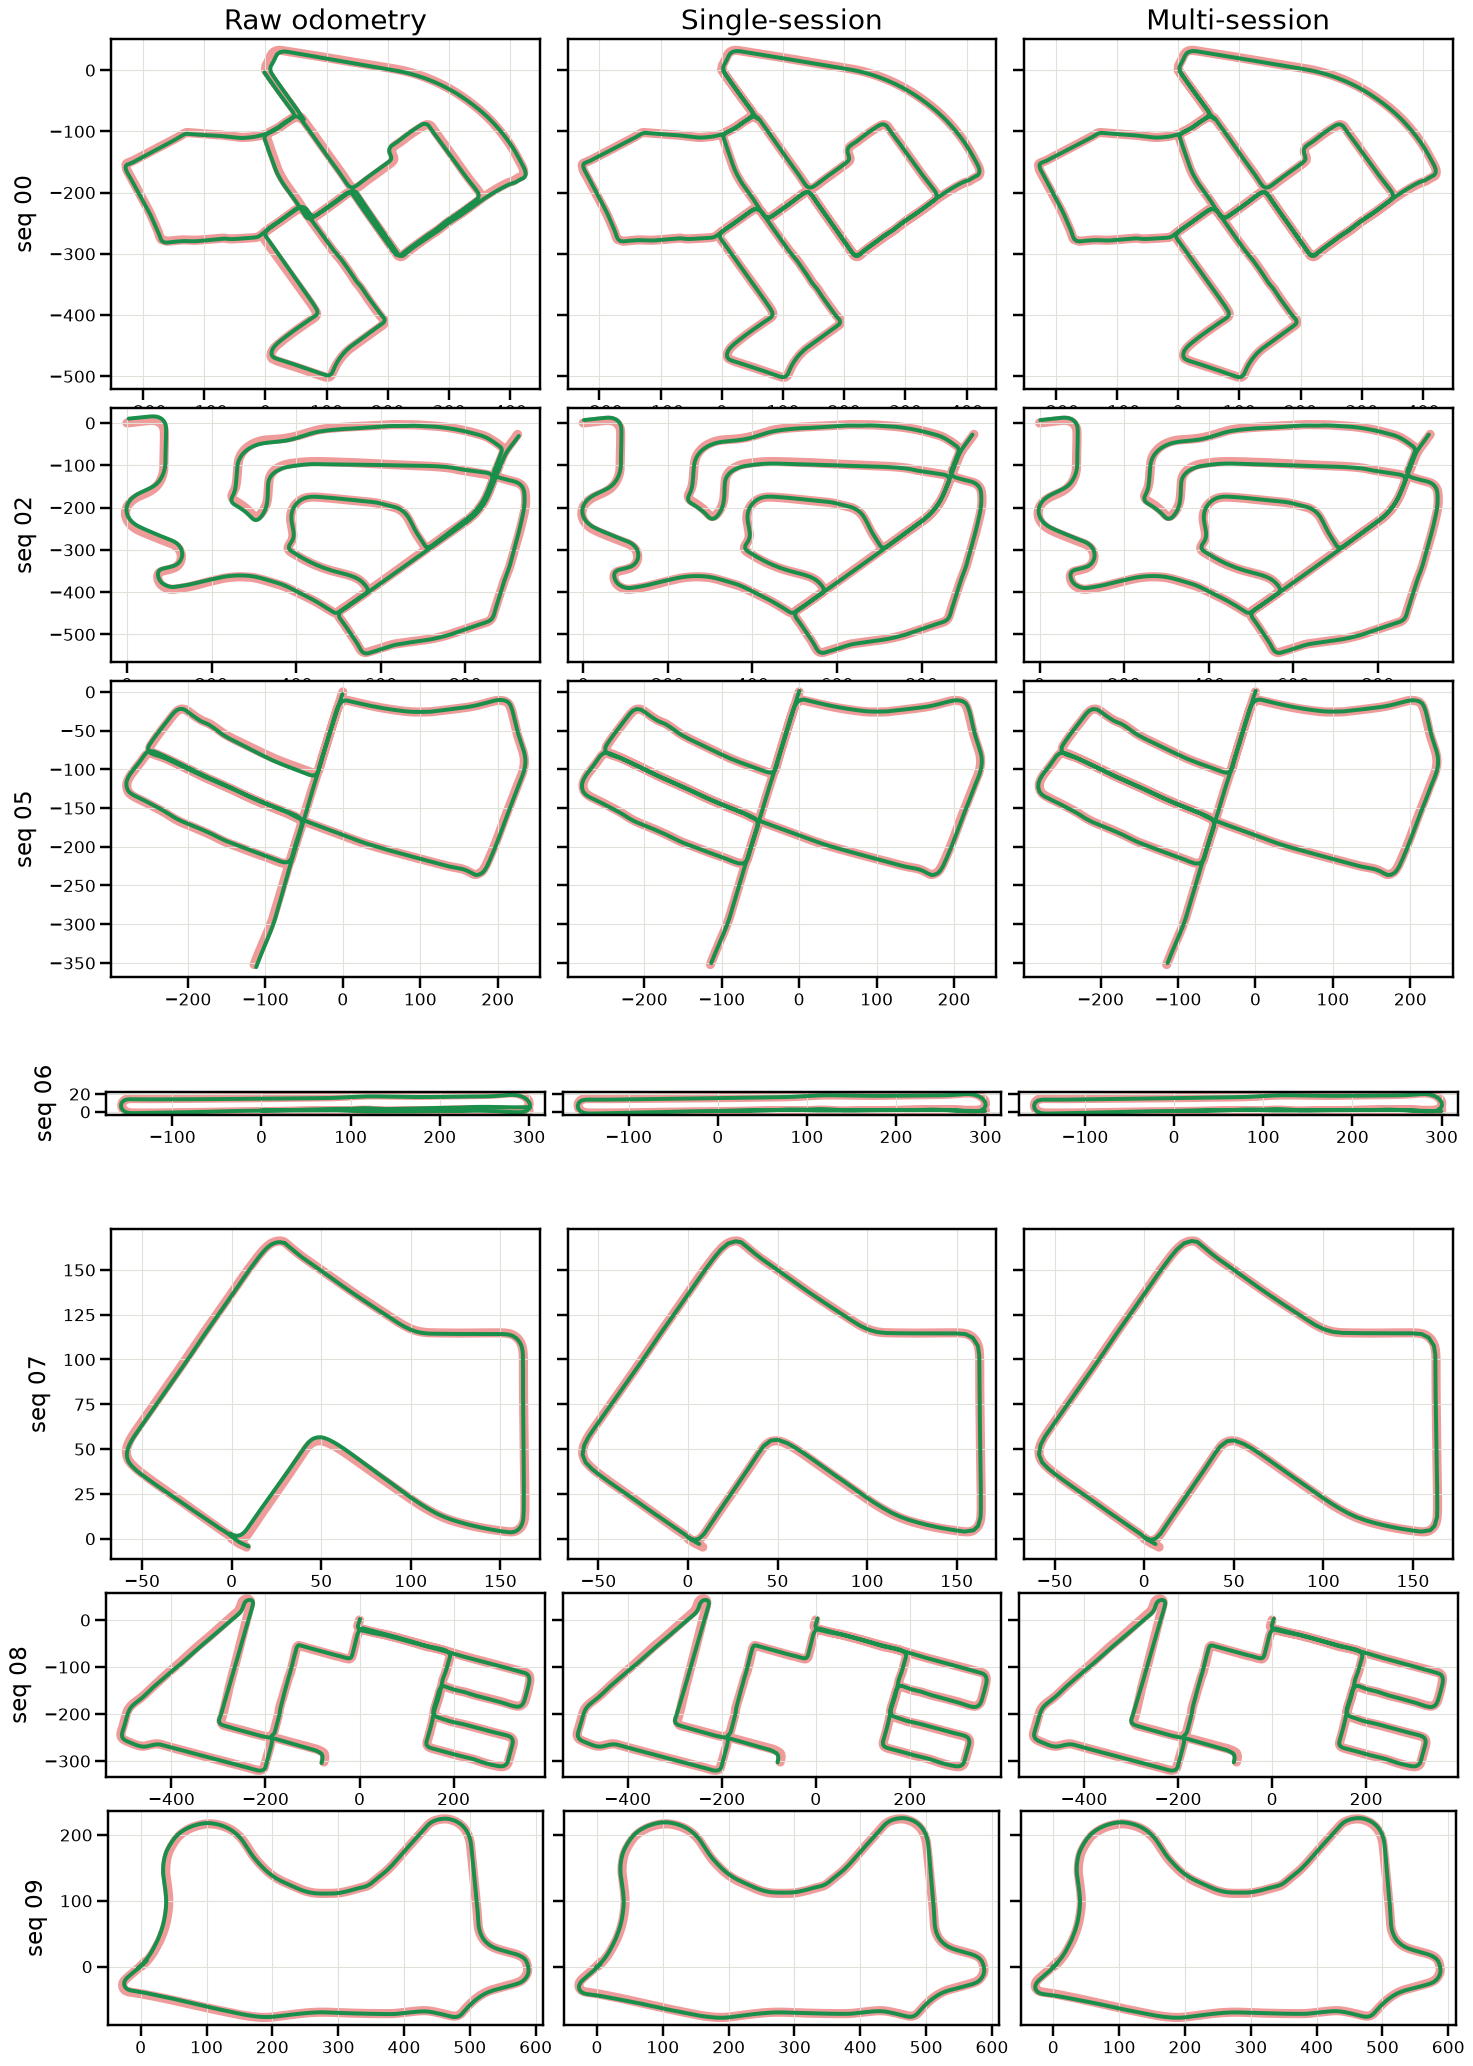
\includegraphics[width=0.9\textwidth]{images/07_appendix/kitti_grid_orb.png}
  \caption[KITTI trajectory grid, ORB-SLAM3 backbone]{KITTI trajectory grid, ORB-SLAM3 backbone,
    all 7 loop-closure sequences: raw odometry, single-session, and multi-session output
    (green) against GT (red), GT-aligned.}
  \label{fig:appendix-kitti-orb}
\end{figure}

\begin{figure}[htbp]
  \centering
  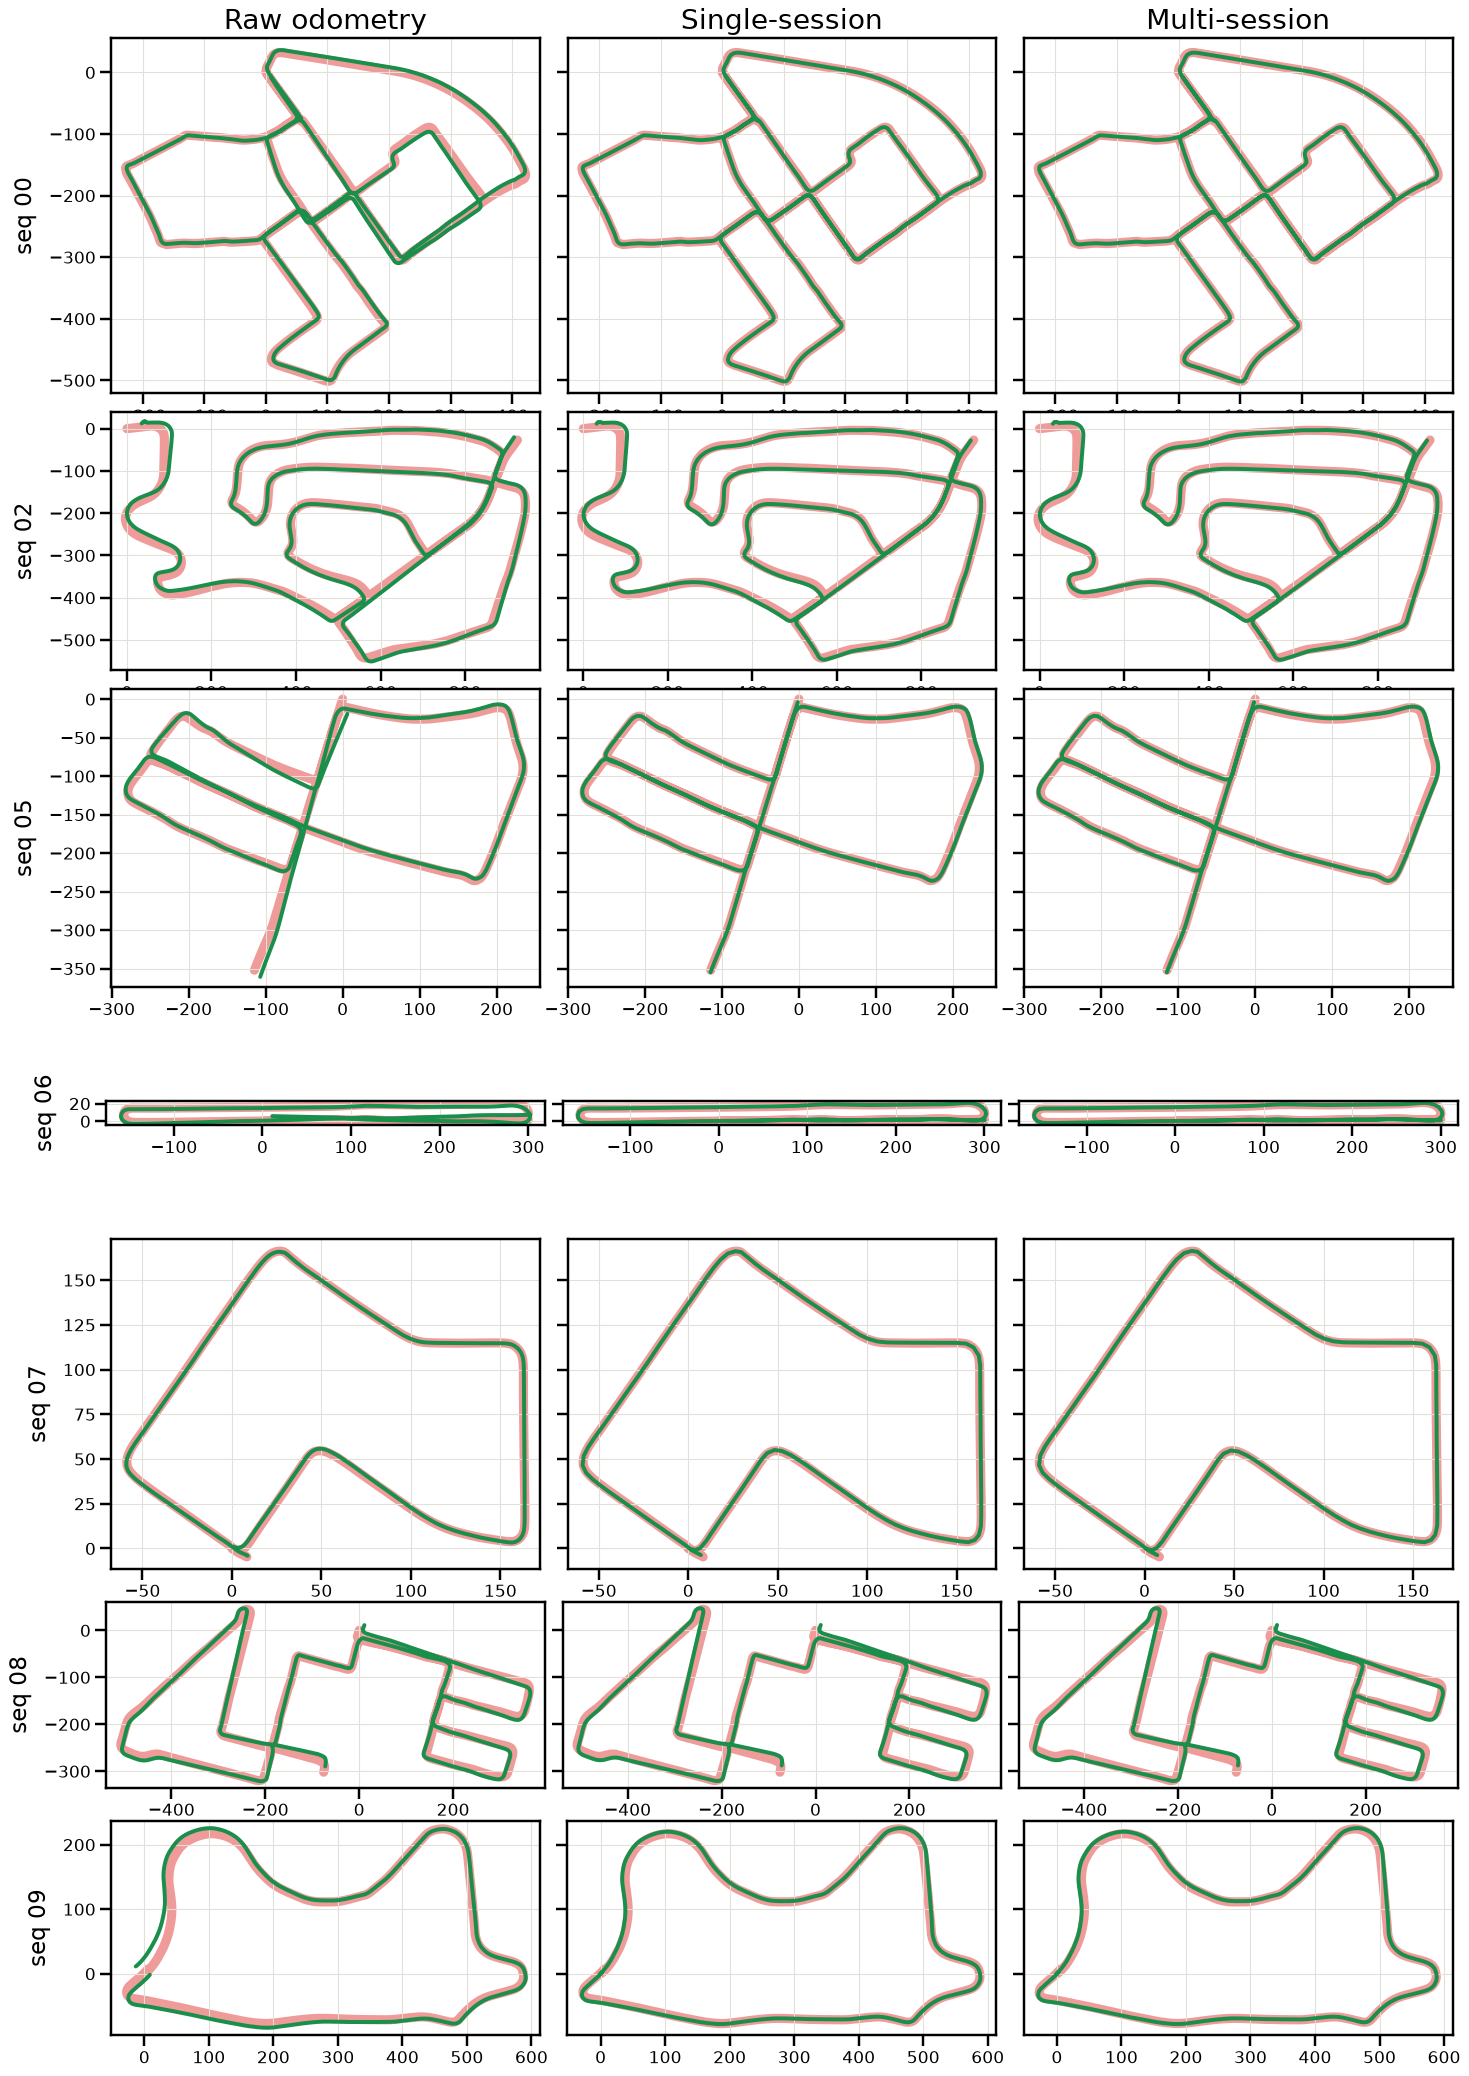
\includegraphics[width=0.9\textwidth]{images/07_appendix/kitti_grid_vins.png}
  \caption[KITTI trajectory grid, VINS-Fusion backbone]{Same layout as
    \myfigref{fig:appendix-kitti-orb}, VINS-Fusion backbone. Sequence 08's raw odometry visibly
    drifts from GT and stays uncorrected in both the single- and multi-session columns, the same
    drift pattern in all three panels (\mytabref{tab:experiments-kitti-vins}'s detection-miss
    caveat: zero intra- or cross-session edges found for this sequence on this backbone).}
  \label{fig:appendix-kitti-vins}
\end{figure}

\section{HGE Trajectory Comparison}
\label{sec:appendix-hge-traj}

\begin{figure}[htbp]
  \centering
  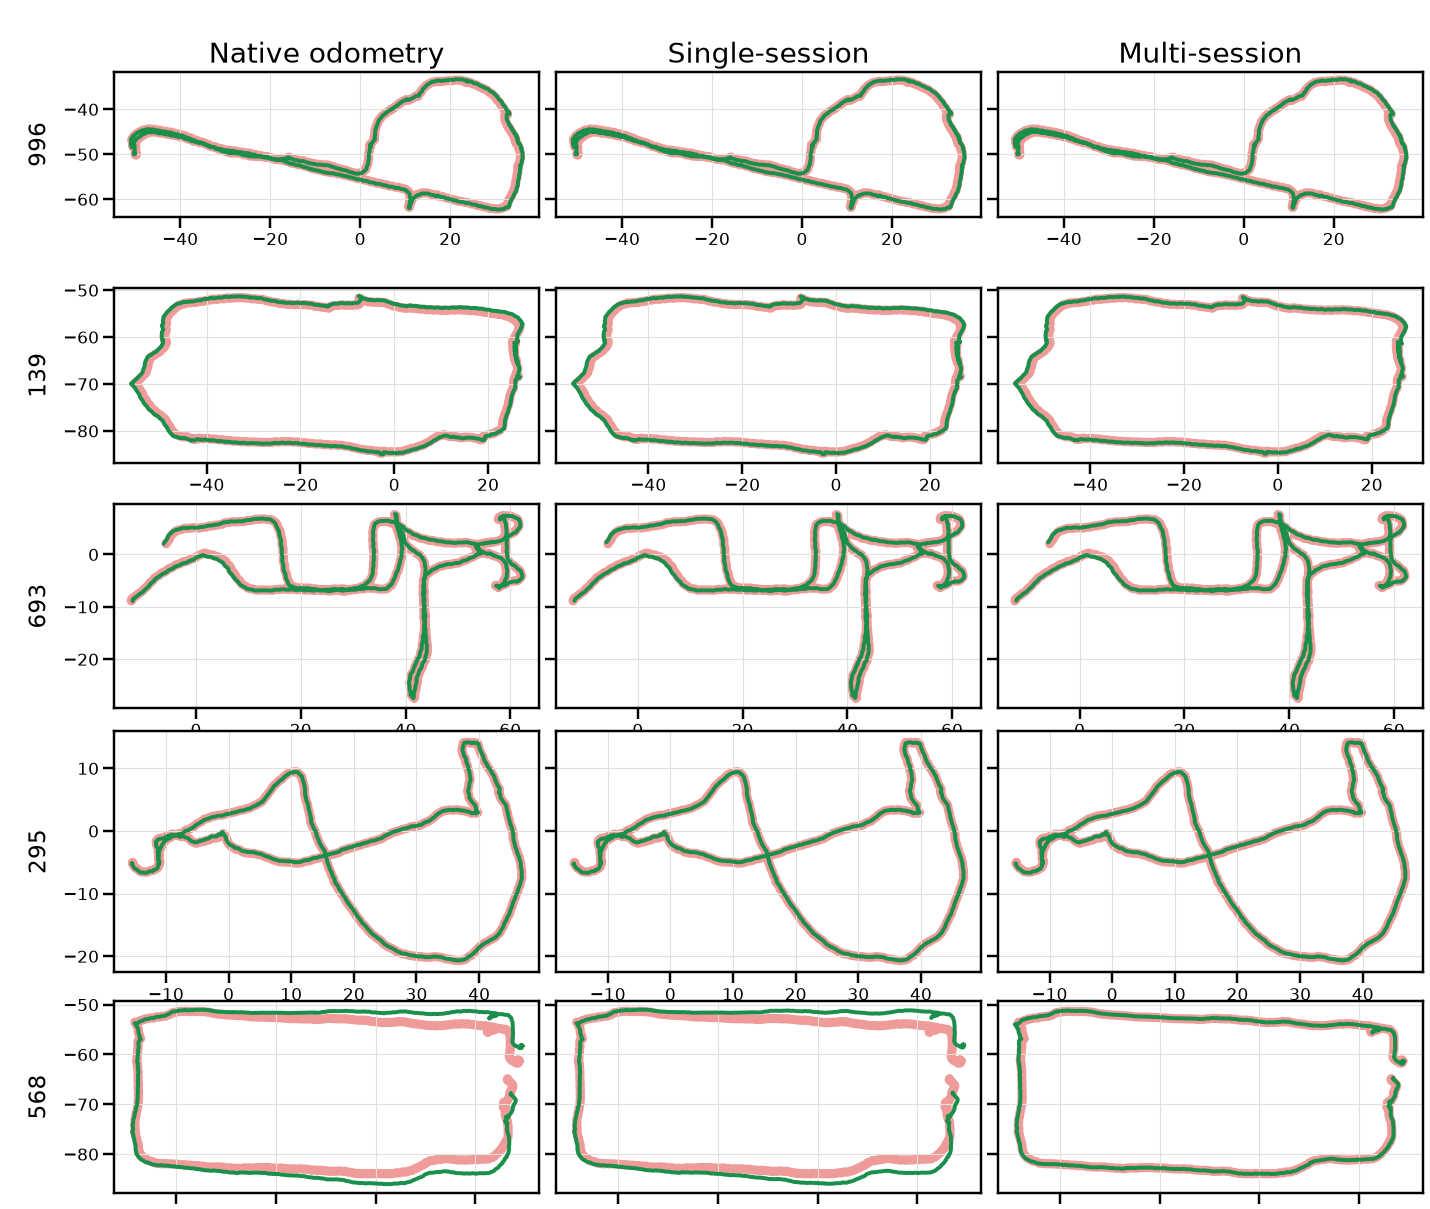
\includegraphics[width=0.9\textwidth]{images/07_appendix/hge_hololens_grid.png}
  \caption[HGE trajectory grid, HoloLens sessions]{HGE trajectory grid, HoloLens sessions
    (device-isolated \texttt{hl\_split} run): native odometry, single-session, and multi-session
    output (green) against GT (red), GT-aligned. Session \texttt{568}'s native odometry drifts
    heavily and is visibly corrected in the multi-session column, matching \mytabref{tab:experiments-hge-ate}'s
    2.09\,m $\to$ 0.29\,m improvement.}
  \label{fig:appendix-hge-hololens}
\end{figure}

\begin{figure}[htbp]
  \centering
  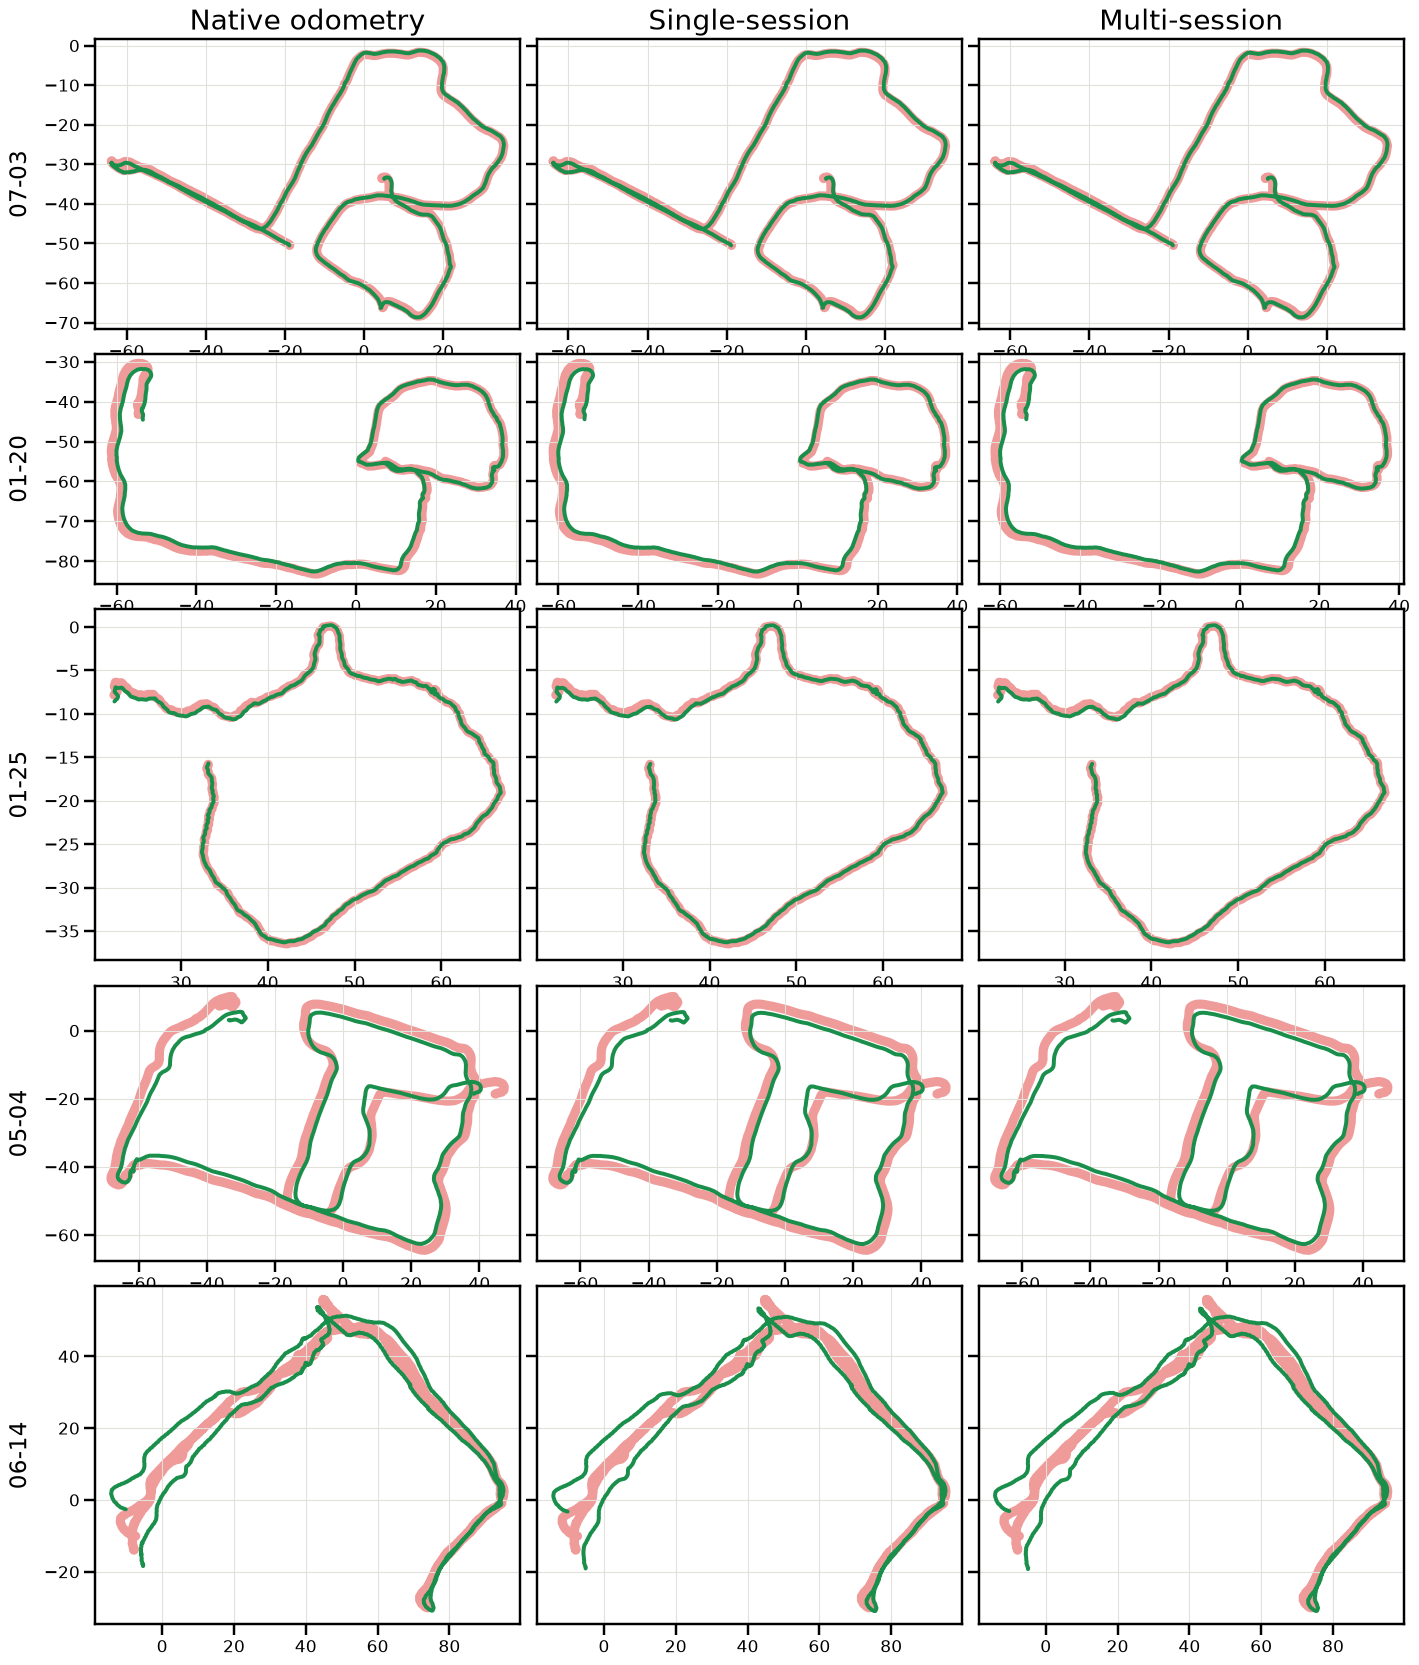
\includegraphics[width=0.9\textwidth]{images/07_appendix/hge_ios_grid.png}
  \caption[HGE trajectory grid, iOS sessions]{Same layout as \myfigref{fig:appendix-hge-hololens},
    the 4 iOS/ARKit sessions of the device-isolated \texttt{ios\_split} run
    (\mytabref{tab:experiments-hge-mixed}'s real 4-session iOS list, not the older 5-session pick
    behind \mysecref{sec:experiments-hge}'s Datasets-section figure).}
  \label{fig:appendix-hge-ios}
\end{figure}

\section{HYDRO Trajectory Comparison}
\label{sec:appendix-hydro-traj}

\begin{figure}[htbp]
  \centering
  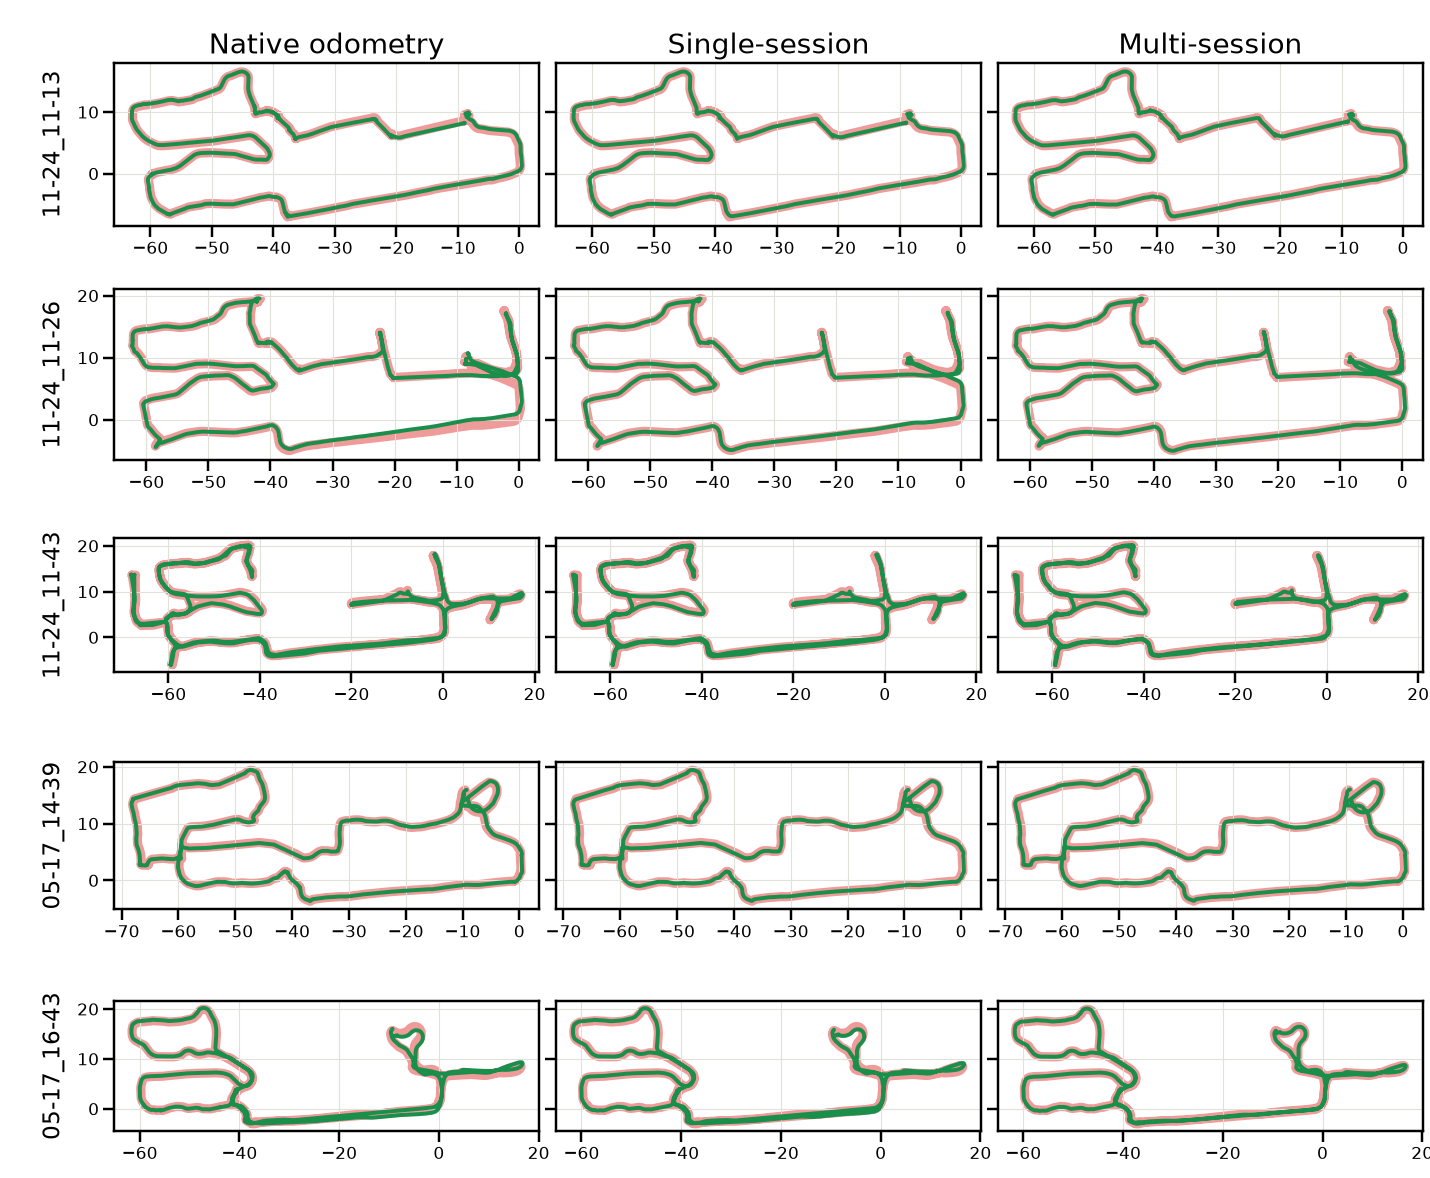
\includegraphics[width=0.9\textwidth]{images/07_appendix/hydro_grid.png}
  \caption[HYDRO trajectory grid]{HYDRO trajectory grid, all 5 sessions, same layout as
    \myfigref{fig:appendix-hge-hololens}. All 5 sessions form one connected component
    (\mytabref{tab:experiments-hydro-ate}).}
  \label{fig:appendix-hydro-traj}
\end{figure}

\section{HYDRO Ref-Anchoring Visualization}
\label{sec:appendix-hydro-anchor}

\begin{figure}[htbp]
  \centering
  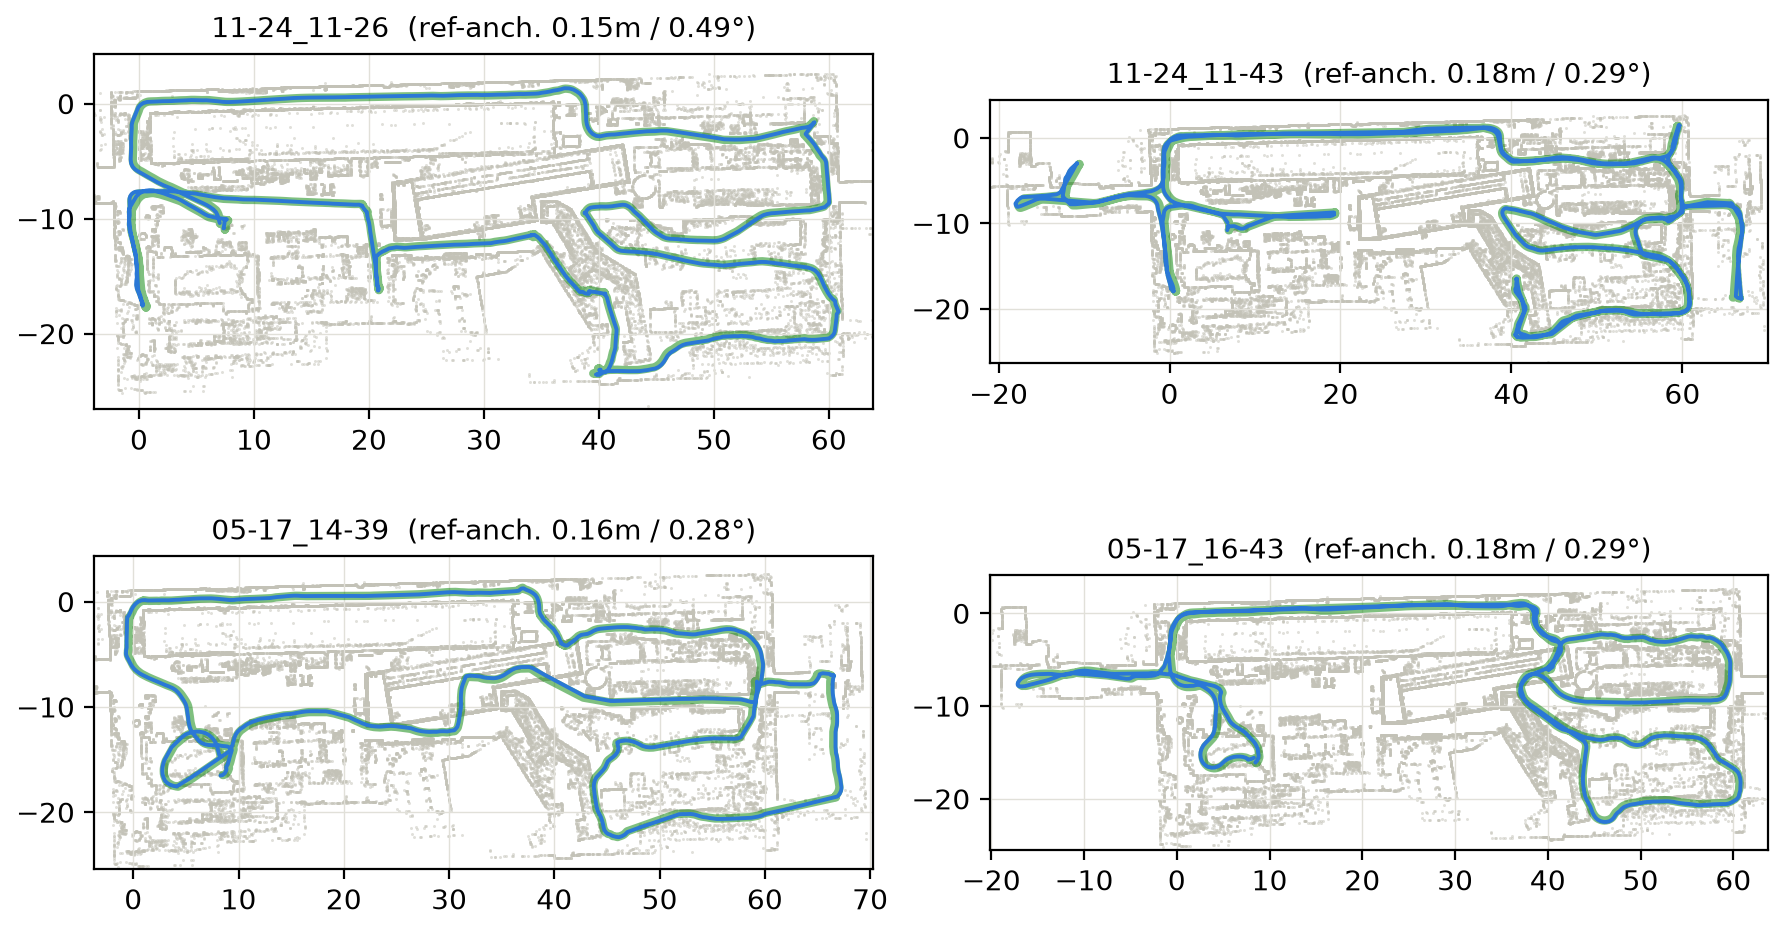
\includegraphics[width=\textwidth]{images/07_appendix/hydro_anchor_individual.png}
  \caption[HYDRO ref-anchored estimate vs.\ GT, per session]{HYDRO's 4 non-reference sessions,
    each panel showing that session's ref-anchored estimate (blue) against its own GT (green,
    faded), over the real site-scan floor plan. Same methodology as
    \texttt{pipelines/compute\_ref\_anchored.py} (\mytabref{tab:experiments-hydro-ate}'s
    ref-anchored columns): the reference session (\texttt{11-24\_11-13}) is Umeyama-fit to its
    own GT once, and that same fixed transform, not an independent per-session fit, is applied to
    every other session's estimate before comparing it to its own GT.}
  \label{fig:appendix-hydro-anchor-individual}
\end{figure}

\begin{figure}[htbp]
  \centering
  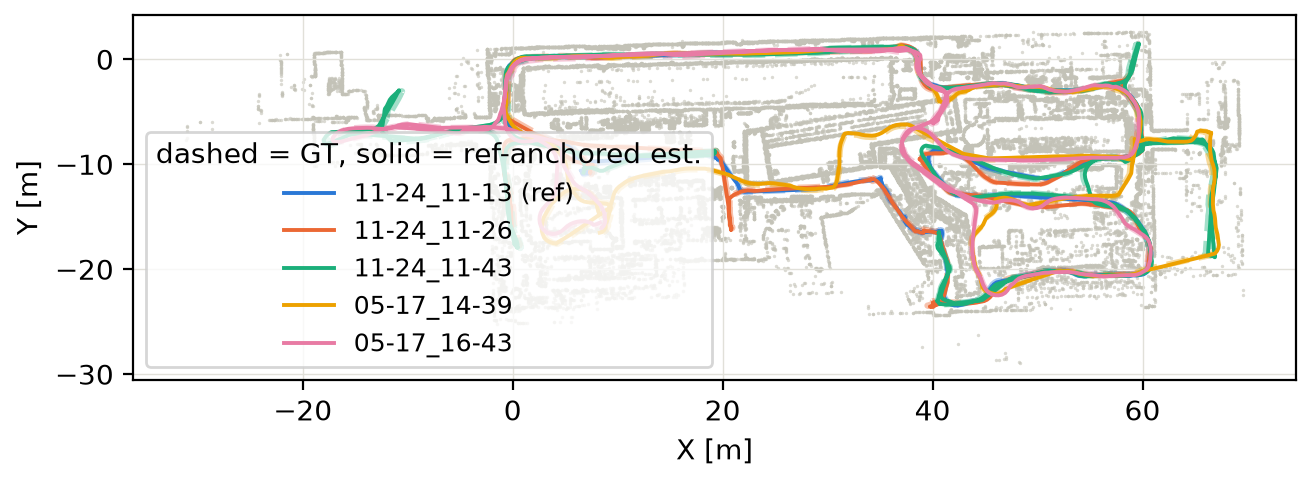
\includegraphics[width=\textwidth]{images/07_appendix/hydro_anchor_combined.png}
  \caption[HYDRO ref-anchored estimates, all sessions combined]{All 5 HYDRO sessions in one
    shared frame: dashed lines are each session's own GT, solid lines its ref-anchored estimate,
    same color per session, same real floor-plan backdrop as \myfigref{fig:appendix-hydro-anchor-individual}.
    Visualizes the same 0.15--0.18\,m ref-anchored translation error that
    \mytabref{tab:experiments-hydro-ate} reports numerically.}
  \label{fig:appendix-hydro-anchor-combined}
\end{figure}
